\documentclass[unknownkeysallowed,xcolor=table]{beamer}
 
\usepackage[T2A,T1]{fontenc}
\usepackage[utf8]{inputenc}
\usepackage[english,russian]{babel}
\usepackage{amsmath}
\usepackage{listings}
\usepackage{url}
\usepackage{textcomp}
\usepackage{multirow}
\usepackage{tikz}

\setbeamertemplate{navigation symbols}{}

\newcommand{\textapprox}{\raisebox{0.5ex}{\texttildelow}}

\newcommand{\rarr}{$\rightarrow$}
 
\colorlet{mygreen}{green!60!blue}
\colorlet{mymauve}{red!60!blue}
\definecolor{light-gray}{gray}{0.9}

\lstset{
      basicstyle=\ttfamily\small,
      commentstyle=\color{mygreen},
      keywordstyle=\color{blue},
      numberstyle=\tiny\color{blue},
      stringstyle=\color{mymauve},
      numbers=left,
      stepnumber=1,
      columns=fullflexible,
      breaklines=true,
      postbreak=\mbox{\textcolor{red}{\ensuremath{\hookrightarrow}\space}},
      literate={~} {\textapprox}{1},
      language={[11]C++}
}

\lstnewenvironment{cmdline}
  {\lstset{
      basicstyle=\ttfamily\scriptsize,
      keywordstyle=\color{blue},
      backgroundcolor=\color{light-gray},
      language={bash}
  }}
  {}

\lstnewenvironment{cmdlinelarge}
  {\lstset{
      basicstyle=\ttfamily\small,
      keywordstyle=\color{blue},
      backgroundcolor=\color{light-gray},
      language={bash}
  }}
  {}

\makeatletter
\newcommand{\srcmediumsize}{\@setfontsize{\srcmediumsize}{7pt}{7pt}}
\makeatother

\makeatletter
\newcommand{\srcbigsize}{\@setfontsize{\srcbigsize}{8pt}{8pt}}
\makeatother

\makeatletter
\newcommand{\srcsize}{\@setfontsize{\srcsize}{6pt}{6pt}}
\makeatother

\makeatletter
\newcommand{\srcsmallsize}{\@setfontsize{\srcsmallsize}{5pt}{5pt}}
\makeatother

\title[C++]
{Программирование на языке C++}
 
\subtitle{Вводный курс}
 
\author[А.~Б.~Морозов]
{
  \texorpdfstring{Александр Морозов\newline\href{mailto:gelu.speculum@gmail.com}{gelu.speculum@gmail.com}}
  {Александр Морозов}
}
  
\date[ITMO 2020]
{ИТМО, весенний семестр 2020}
 
\logo{%
  \makebox[0.97\paperwidth]{%
    
\includegraphics[align=c,width=2cm,keepaspectratio]{itmo_logo.png}
    \hfill
    
\includegraphics[align=c,width=1.5cm,keepaspectratio]{itiviti_logo.png}
  }
}

\AtBeginSection[]
{
  \begin{frame}
    \frametitle{Содержание}
    \tableofcontents[currentsection]
  \end{frame}
}

\begin{document}
 
\frame{\titlepage}

%-------------------------------------------------
\section{Текст программы и этапы его обработки}

\begin{frame}{Текст программы}
  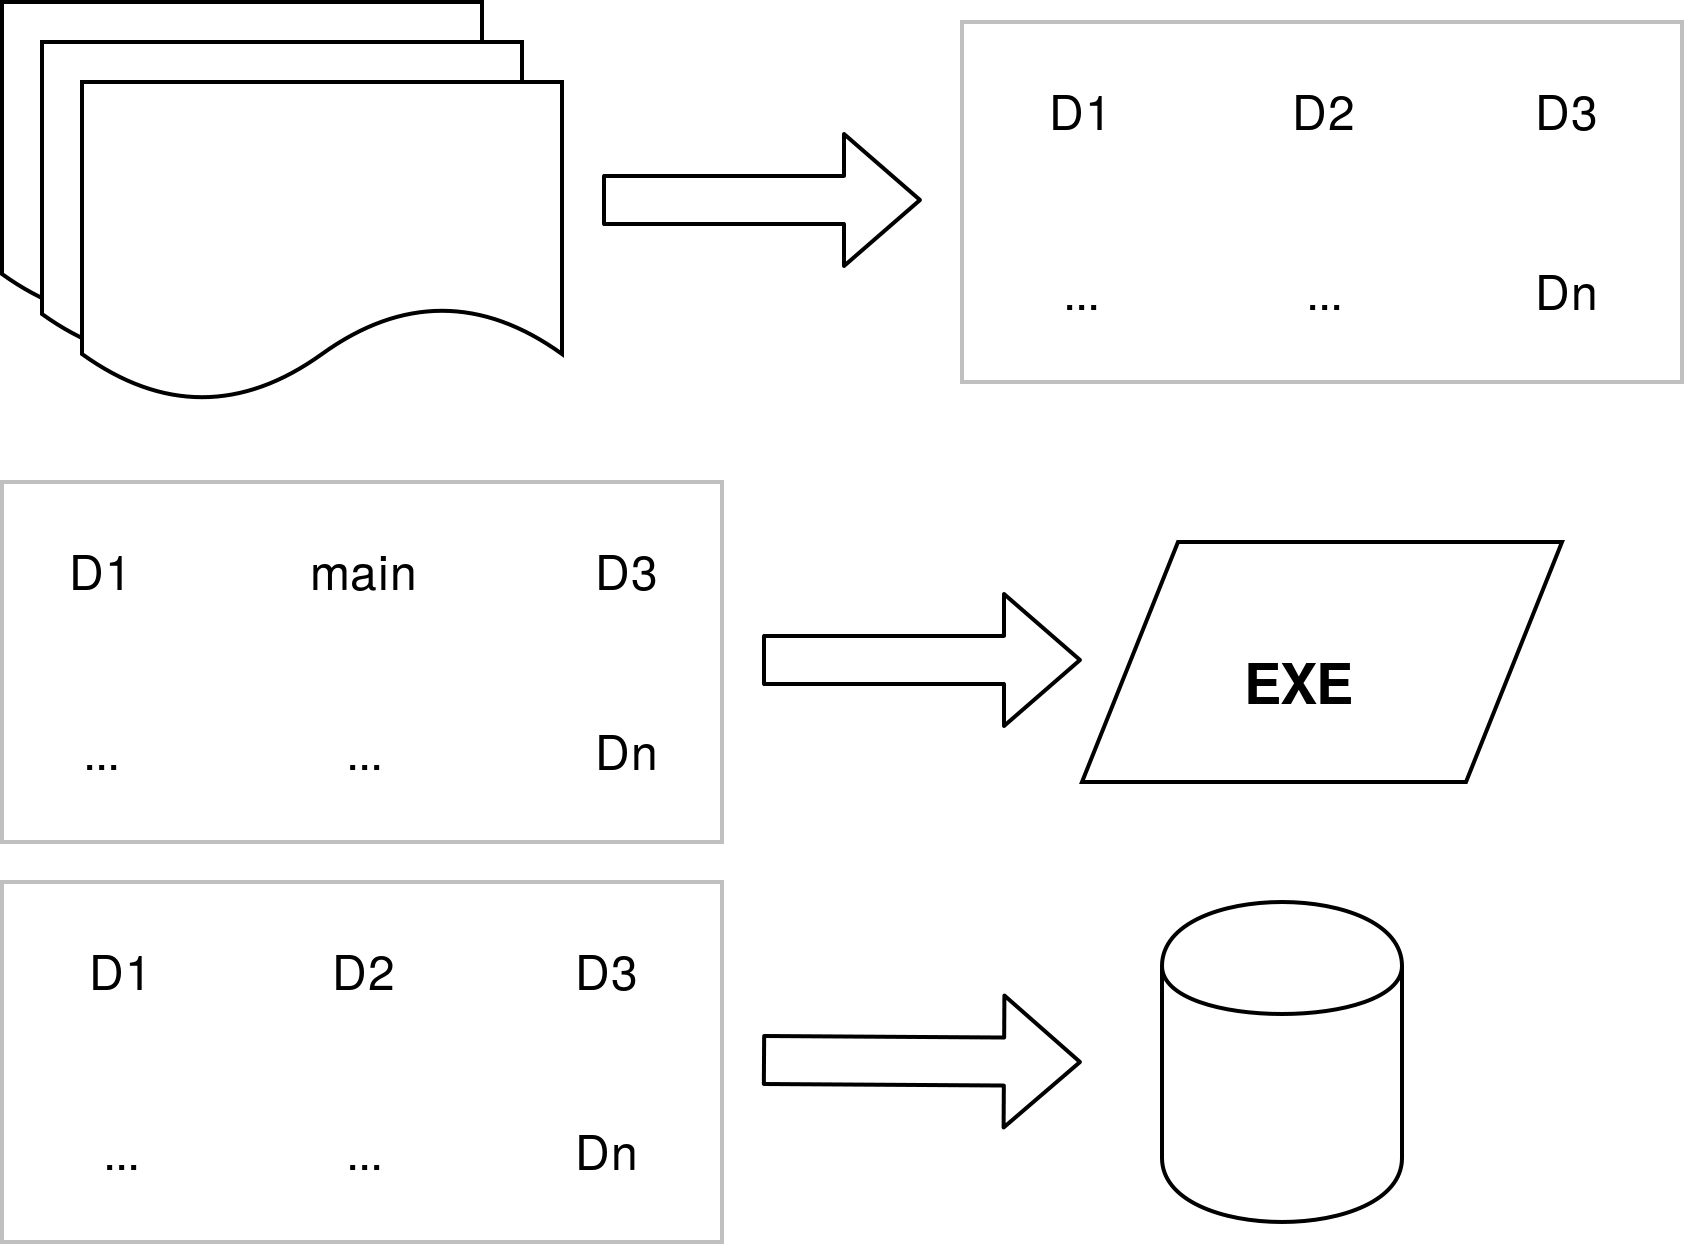
\includegraphics[align=c,width=9.5cm,keepaspectratio]{images/text_decl_bin.png}
\end{frame}

\begin{frame}[fragile]{Комментарии}
  \begin{lstlisting}
  /* Comment */

  /*
   * Multi-line comment
   */

  // Single-line comment

  //
  //
  // Fancy comment formatting
  //
  \end{lstlisting}
\end{frame}

\begin{frame}[fragile]{Основные этапы трансляции}
  \begin{enumerate}
    \item Склейка строк через \lstinline{\} \vspace{1em}
    \item Предварительная токенизация (комментарии, пробелы, базовые токены) \vspace{1em}
    \item Препроцессор ($\forall I \rightleftharpoons 1\dotso3$) \vspace{1em}
    \item Склейка смежных строковых литералов \vspace{1em}
    \item Компиляция \vspace{1em}
    \item Компоновка
  \end{enumerate}
\end{frame}

\begin{frame}[fragile]{Базовые токены}
  \begin{itemize}
    \item идентификаторы
    \item числовые токены
    \item символьные, строковые литералы и аргументы \lstinline{#include}
    \item операторы и символы пунктуации
    \item иное
  \end{itemize}
  \begin{lstlisting}
    a+++++b   // a ++ ++ + b
    a++ + ++b // a ++ + ++ b
    1E+12 // OK
    0x1E+12 // bad
    0x1E +12 // OK
  \end{lstlisting}
\end{frame}

%-------------------------------------------------
\section{Функция main}

\begin{frame}[fragile]{Функция main}
  \begin{itemize}
    \item нельзя явно вызвать
    \item нельзя взять адрес
    \item не может быть автоматически сгенерирована
    \item не может быть перегружена
    \item не может иметь спецификаторов \lstinline{inline}, \lstinline{static}, \lstinline{constexpr}
  \end{itemize}
  \vspace{1em}
  \begin{lstlisting}
    int main() { /* body */ }
    int main(int argc, char * argv[]) { /* body */ }
  \end{lstlisting}
  \vspace{1em}
  \begin{itemize}
    \item вызывается после инициализации глобальных переменных
    \item выход из \lstinline{main} $\equiv$ завершение программы
    \item \lstinline{return 0;} автоматически генерируется в конце тела
  \end{itemize}
\end{frame}

%-------------------------------------------------
\section{Базовые элементы программы}

\begin{frame}[fragile]{Идентификаторы}
  \begin{itemize}
    \item \lstinline{[A-Za-z_][A-Za-z0-9_]*} \vspace{1em}
    \item совпадающие с ключевыми словами -- зарезервированы \vspace{1em}
    \item содержащие \lstinline{__} -- зарезервированы \vspace{1em}
    \item начинающиеся с \lstinline{_[A-Z]} -- зарезервированы \vspace{1em}
    \item начинающиеся с \lstinline{_} -- зарезервированы в глобальном пространстве имён
  \end{itemize}
\end{frame}

\begin{frame}[fragile]{Неквалифицированные идентифицирующие выражения}
  \begin{itemize}
    \item корректно определённые идентификаторы \vspace{0.5em}
    \item имя перегруженного оператора \lstinline{operator ==} \vspace{0.5em}
    \item имя оператора пользовательского преобразования типа \lstinline{operator bool} \vspace{0.5em}
    \item имя оператора пользовательского литерала \lstinline{operator "" _km} \vspace{0.5em}
    \item имя шаблона со списком аргументов \lstinline{T<a, b, c>} \vspace{0.5em}
    \item символ \lstinline{~} с последующим именем класса \lstinline{~Foo} \vspace{0.5em}
    \item \lstinline{~decltype(x)}
  \end{itemize}
\end{frame}

\begin{frame}[fragile]{Квалифицированные идентифицирующие выражения}
  \begin{lstlisting}
    int a = 13;

    struct C
    {
      int get() const
      { return a; }

      int get2() const
      { return ::a; }

      int get3() const
      { return ::C::a; }

      static int a = 111;
    };

    int b = C::a;
  \end{lstlisting}
\end{frame}

\begin{frame}[fragile]{Имена}
  Имя -- идентифицирующее выражение, связанное с некой программной сущностью через определение. \vspace{2em}
  \begin{lstlisting}
    int a = 1; // declaration

    int f()
    {
        return a; // usage
    }
  \end{lstlisting}
  \vspace{2em}
  Использование \rarr поиск имён \rarr сущность
\end{frame}

\begin{frame}[fragile]{Литералы}
  \begin{itemize}
    \item булевские \lstinline{true}, \lstinline{false}
    \item целочисленные
    \item дробные
    \item символьные
    \item строковые
    \item \lstinline{nullptr}
  \end{itemize}
\end{frame}

\end{document}
